\documentclass[../../main.tex]{subfiles}

    \lstset{basicstyle=\small,
      showstringspaces=false,
      commentstyle=\color{black},
      keywordstyle=\color{blue}
    }

    \graphicspath{{images/}{../../images/}}

    \begin{document}
    \subsection{Akustik}
    Während der Fahrt wird von einer Tafel die Zahl abgelesen, diese soll am Ende akustisch wiedergegeben werden.
    In diesem Abschnitt werden verschiedene akustische Lösungsansätze/Konzepte zusammengetragen und verglichen.
    Ziel ist es aus einem breiten Spektrum die optimale Lösung zu finden.\\
    \\

    \subsubsection{Anforderung}
    Die Software muss in der Lage sein eine Zahl zwischen 1 und 9, welche als Parameter übergeben wird, akustisch wieder zu geben.
    Ausgabe muss verständlich und darf nicht zu laut sein.\\
    \\

    \subsubsection{Auswahl Konzepte Software}
    In disem Kapitel werden verschiedene Softwarekonzepte zusammengetragen. Bei den Programmiersprachen habe ich mich für Python
    und Java entschieden, da diese erstklassige Kandidaten für unsere Systemsteuerung sind.
    Somit wird ein reibungsloses Zusammenspiel gewährleistet.\\

    Es wurde ausschliesslich Freeware benutzt um unser Budget zu schützen und weil diese ausreichende Funktionalität mit sich bringen.

    \textbf{Python pygame}\\
    Die python Bibliothek 'pygame' erlaubt es dem Benutzer relativ einfach Audiodateien abzuspielen.
    Dies geschieht über einen integrierten Mixer, welche auf mehreren Spuren gleichzeitig Musik abspielen kann.
    Für diese Aufgabe reicht bereits eine Tonspur.\\

    Das ganze sieht dann folgendermassen aus (acoustic.py):
    \begin{lstlisting}
    mixer.init() #turn all of pygame on.
    mixer.music.set_volume(0.5)

    mixer.music.load('Soundfiles/E9.mp3')
    mixer.music.play()
    #play() is asynchronous and will stop as soon as the programm ends
    time.sleep(2)
    mixer.music.stop()
    \end{lstlisting}

    Weil die Tonspur asynchron abgespielt wird, muss man nach dem Aufruf 'play()' eine Zeit warten, bis das Stück zu Ende gespielt hat.
    Dies erweist sich als relativ ungünstig, denn die Stücke sind nicht alle gleich lang.

    Einfach zu bedienende Python Bibliothek mit netten Features, jedoch nicht für unseren Gebrauch geignet.\\

    \textbf{Python pyttsx3}\\
    Bei der python Bibliothek 'pyttsx3' handelt es sich um einen 'Text To Speech'(Deutsch: Text zu Sprache) converter.
    Dieser ermöglicht das Übersetzen von Text zu Sprache in Echtzeit und bringt hiermit eine enorme Flexibilität mit sich.
    Das ganze ist einfach zu bedienen und erlaubt die Ausgabe über mehrere Sprachen.\\

    Das ganze sieht dann folgendermassen aus (acousticTTS.py):
    \begin{lstlisting}
    engine = pyttsx3.init()
    engine.say('Number ' + str(number))
    engine.runAndWait()
    \end{lstlisting}

    Extrem simpel und übersichtliche Ausführung (nur 3 Zeilen). Ausgabe ist sehr verständlich.\\
    Sehr gelungene Bibliothek.

    \textbf{Java Media}\\
    Mit den Java Media Bibliotheken kann man verschiedene Audioformate ausgeben.
    Benötigt werden die Importe 'Media' und 'MediaPlayer' aus der 'javafx.scene.media' Umgebung.
    Zusätlich muss noch von der 'Application' Klasse geerbt werden und der Befehl 'Application.launch()' ausgeführt werden.
    Die kommt dadurch, dass 'javafx' eine verborgene Initialisierung benötigt,
    welche am einfachsten über 'Application.launch()' gestartet wird.\\

    Das sieht dann folgendermassen aus (acoustic.java):
    \begin{lstlisting}
    Application.launch();
    String filePath = System.getProperty("user.dir") + "/Soundfiles/E9.wav";

    File soundFile = new File(filePath);
    Media hit = new Media(soundFile.toURI().toString());
    MediaPlayer mediaPlayer = new MediaPlayer(hit);
    mediaPlayer.play();
    \end{lstlisting}

    Einfach zu bedienende Bibliothek mit kleiner Umständlichkeit.

    \textbf{}{Java FreeTTS}
    Java FreeTTS besteht aus verschiedenen 3. Party Bibliotheken.
    Leider hatte ich keinen Erfolg die Applikation funktionsfähig zu machen.

    \subsubsection{Auswahl Konzepte Hardware}
    In diesem Kapitel werden einige Hardware Konzepte vorgestellt.
    Wir unterscheiden hier zwischen 3 Varianten, wie Audio ausgegeben wird.
    Daher würden auch Änderungen an der Softwarelösung vorgenommen werden müssen.

    \textbf{Speaker}\\
    Bei dieser Lösung wird der Ton direkt von der Software über einen Lautsprecher ausgegeben.
    Dies ist die meist verbreitete Lösung.\\

    \textbf{Buzzer}\\
    Der Buzzer wird über die selbe Hardwareinheit wie der Speaker realisiert, mit dem einzigen
    Unterschied, dass man über eine integrierte Komponente den Speaker zum 'buzzen' nutzt.

    \textbf{Speaker with DataStorage}\\
    Der Speaker vefügt zusätzlich über einen integrierten Datenspeicher, über welchen Audiodateien abgespeichert
    und auf Befehl abgespielt werden können. Dies hat zur Folge, dass Softwaretechnisch Zeit und Ressourcen gespart werden können.

    \subsubsection{Nutzwertanalyse}
    Konzepte werden zusammengetragen und verglichen.
    In den verschiedenen Disiplinen werden Wertungen von 1 - 5 abgegeben, wobei 1 die schlechteste und 5 die beste Wertung ist.
    Auch wird auf spezifische Stärken und Schwächen eingegangen.

    \textbf{NutzwertanalyseSoftware:}\\
    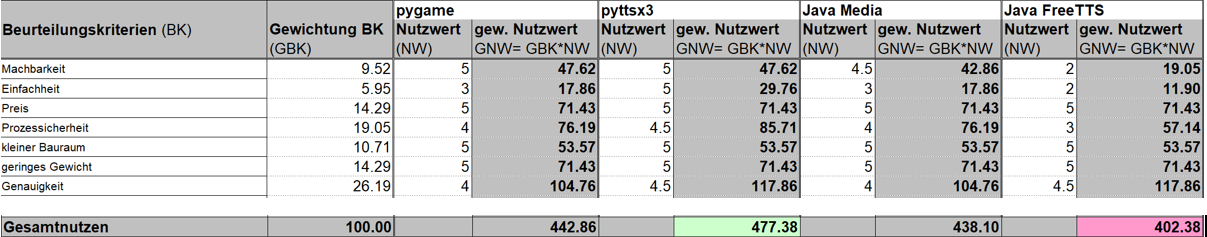
\includegraphics{Akustik/NutzwertanalyseAkustikSoftware}
    \paragraph{Entscheidung}
    Favoriten sind die beiden Python Bibliotheken, jedoch macht es Sinn, dass wir für erhöhte Flexibilität von jeder Sprache einen Favoriten festlegen. Dies erlaubt uns später jederzeit zwischen den Konzepten zu wechseln.

    \textbf{NutzwertanalyseSoftware:}\\
    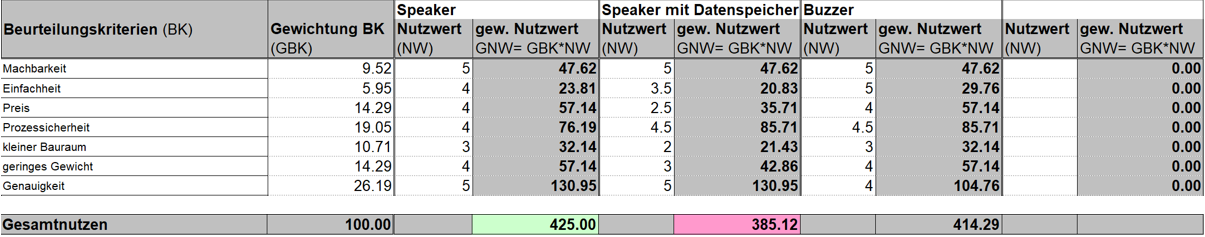
\includegraphics{Akustik/NutzwertanalyseAkustikHardware}
    \paragraph{Entscheidung}
    Weil der Speaker das meist verbreitete und praktischste Ausgabemittel für Audioaufnahmen ist, werden wir uns mit diesem versuchen.
    Sollten wir keinen Erfolg erzielen, werden wir der Einfachheit wegen zum Buzzer ausweichen.


  \end{document}
